\documentclass[letterpaper,oneside,12pt]{report}

\usepackage[spanish]{babel} 
\usepackage[T1]{fontenc}
\usepackage[ansinew]{inputenc}
\usepackage{graphicx}
\usepackage{amsmath}
\usepackage{amsthm}
\usepackage{amsfonts}
\onehalfspacing  
\begin{document}

\pagestyle{empty} 

\title{Fundamentos del M\'etodo de Rigideces}

\author{Dr. Jorge H. Ch\'avez G\'omez}
\date{Enero 2013}
\maketitle
\addtocontents{toc}{\protect\vspace*{\baselineskip}}

\section{Estructura Analizada.}

\paragraph{} La estructura analizada durante la clase del 21 de enero de 2013 se reproduce a continuaci\'on en la Figura\ref{fig:fig1} la cual corresponde a una viga de tres apoyos sujeta a una carga uniformemente distribuida en su primer claro.

\begin{figure}[htbp]
  \centering
		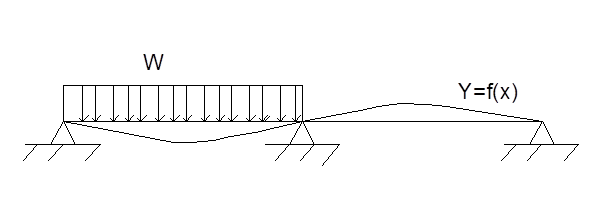
\includegraphics[scale=0.7]{fig1.png}
	\caption{Estructura Hiperest\'atica de Estudio.}
	\label{fig:fig1}
\end{figure}

\paragraph{} La energia total del sistema ser\'a funci\'on de la energ\'{\i}a interna y la energ\'{\i}a externa como a continuaci\'on. 
$$U=\frac{1}{2}\int_{L_{t}}{M_{X}Y^{''}dx}=\frac{1}{2}\int_{L_{t}}{EI(Y^{''})^{2}dx}$$ \\
$$W=\int_{L_{t}}{W_{X}Ydx}$$ \\


\begin{equation}
\Pi=W-U=\int_{L_{t}}{W_{X}(\sum{Y_{i}\overline{Y_{i}})}dx}-\frac{1}{2}\int_{L_{t}}{EI(\sum{Y_{i}^{''}\overline{Y_{i}})^{2}dx }
\quad
\end{equation}


\paragraph{} El proceso natural en el cual una estructura llega a la estabilidad tiende a mantener el m\'{\i}nimo de energ\'{\i}a, es por esto que la expresi\'on de $\Pi$ deber\'a minimizarse a trav\'es de los valores extremos de su expresi\'on; derivando.

$$\frac{\delta\Pi}{\delta\overline{Y_{i}}}=\int_{L_{t}}{W_{X}Y_{i}dx}-\int_{L_{t}}{EI(\sum{Y_{i}^{''}\overline{Y_{i}})(\sum{Y_{i}^{''})dx }$$

\paragraph{} El segundo t\'ermino de la expresi\'on anterior se desarrolla a continuaci\'on:

$$\begin{array}{l}
	(\sum{Y_{i}^{''})(\sum{Y_{i}^{''}\overline{Y_{1}})
	\\ \\ =(Y_{1}^{''}\overline{Y_{1}}+Y_{2}^{''}\overline{Y_{2}}+Y_{3}^{''}\overline{Y_{3}})(Y_{1}^{''}+Y_{2}^{''}+Y_{3}^{''}) 
	\\ \\ ={Y_{1}}^{''}^{2}\overline{Y_{1}}+Y_{1}^{''}\overline{Y_{2}^{''}}\overline{Y_{1}}
	\\ \\ +Y_1^{''}Y_{3}^{''}\overline{Y_{1}}+Y_{1}^{''}Y_{2}^{''}\overline{Y_{2}}+Y_{2}^{''}^{2}\overline{Y_{2}}
	\\ \\ +Y_{2}^{''}Y_{3}^{''}\overline{Y_{2}}+Y_{3}^{''}Y_{1}^{''}\overline{Y_{3}}+Y_{3}^{''}Y_{2}^{''}\overline{Y_{3}}
\\ \\ +Y_{3}^{''}^{2}\overline{Y_{3}}=\sum_{i}\sum_{j}(Y_{i}^{''}Y_{j}^{''}\overline{Y_{i}})
\end{array}$$

\paragraph{} Por el desarrollo anterior se tendr\'a la expresi\'on correspondiente al m\'inimo de \Pi:

\begin{equation}
\frac{\delta\Pi}{\delta\overline{Y_{i}}}=\int_{L_{t}}{W_{X}Y_{i}dx}-\sum_{j}\int_{L_{t}}{EIY_{i}^{''}Y_{j}^{''}\overline{Y_{j}}dx }
\quad
\end{equation}

\paragraph{} De \'esta manera desarrollando los sub\'{\i}ndices de la expresi\'on anterior tendremos para i:

$$\begin{array}{c}
\frac{\delta\Pi}{\delta\overline{Y_{1}}}=\int_{L_{t}}{W_{X}Y_{1}dx}-\sum_{j}\int_{L_{t}}{EIY_{1}^{''}Y_{j}^{''}\overline{Y_{j}}dx }
\\\\
\frac{\delta\Pi}{\delta\overline{Y_{2}}}=\int_{L_{t}}{W_{X}Y_{2}dx}-\sum_{j}\int_{L_{t}}{EIY_{2}^{''}Y_{j}^{''}\overline{Y_{j}}dx }
\\\\
\frac{\delta\Pi}{\delta\overline{Y_{3}}}=\int_{L_{t}}{W_{X}Y_{3}dx}-\sum_{j}\int_{L_{t}}{EIY_{3}^{''}Y_{j}^{''}\overline{Y_{j}}dx }
\end{array}$$

\paragraph{} Desarrollando para satisfacer la condici\'on de los extremos de una funci\'on y as\'{\i} encontrar el valor que minimice la energ\'{\i}a tendremos:

$$\frac{\delta\Pi}{\delta\overline{Y_{i}}}=0$$

\paragraph{} En consecuencia a trav\'es de un proceso de reducci\'on:

$$\begin{array}{c}
\int_{L_{t}}{W_{x}Y_{1}dx}=\int_{L_{t}}{EIY_{1}^{''}Y_{1}^{''}\overline{Y_{1}}dx}+\int_{L_{t}}{EIY_{1}^{''}Y_{2}^{''}\overline{Y_{2}}dx}+\int_{L_{t}}{EIY_{1}^{''}Y_{3}^{''}\overline{Y_{3}}dx}
\\\\
\int_{L_{t}}{W_{x}Y_{2}dx}=\int_{L_{t}}{EIY_{2}^{''}Y_{1}^{''}\overline{Y_{1}}dx}+\int_{L_{t}}{EIY_{2}^{''}Y_{2}^{''}\overline{Y_{2}}dx}+\int_{L_{t}}{EIY_{2}^{''}Y_{3}^{''}\overline{Y_{3}}dx}
\\\\
\int_{L_{t}}{W_{x}Y_{3}dx}=\int_{L_{t}}{EIY_{3}^{''}Y_{1}^{''}\overline{Y_{1}}dx}+\int_{L_{t}}{EIY_{3}^{''}Y_{2}^{''}\overline{Y_{2}}dx}+\int_{L_{t}}{EIY_{3}^{''}Y_{3}^{''}\overline{Y_{3}}dx}
\end{array}$$
\paragraph{} Expresando lo anterior en forma matricial tendremos finalmente:
$$\begin{array}{cccc}
 \begin{Bmatrix}
\int{W_{x}Y_{1}dx}\\\\
\int{W_{x}Y_{2}dx}\\\\
\int{W_{x}Y_{3}dx}\\\\
\end{Bmatrix} & \begin{array}{c} \\=\\ \\ \end{array} & \begin{bmatrix} 
\int_{L_{t}}{EIY_{1}^{''}Y_{1}^{''}\overline{Y_{1}}dx} & \int_{L_{t}}{EIY_{1}^{''}Y_{2}^{''}\overline{Y_{2}}dx} & \int_{L_{t}}{EIY_{1}^{''}Y_{3}^{''}\overline{Y_{3}}dx} \\\\
\int_{L_{t}}{EIY_{2}^{''}Y_{1}^{''}\overline{Y_{1}}dx} & \int_{L_{t}}{EIY_{2}^{''}Y_{2}^{''}\overline{Y_{2}}dx} & \int_{L_{t}}{EIY_{2}^{''}Y_{3}^{''}\overline{Y_{3}}dx} \\\\
\int_{L_{t}}{EIY_{3}^{''}Y_{1}^{''}\overline{Y_{1}}dx} & \int_{L_{t}}{EIY_{3}^{''}Y_{2}^{''}\overline{Y_{2}}dx} & \int_{L_{t}}{EIY_{3}^{''}Y_{3}^{''}\overline{Y_{3}}dx} \\\\ \end{bmatrix} & \begin{Bmatrix} 
\overline{Y_{1}} \\\\
\overline{Y_{2}} \\\\
\overline{Y_{3}} \\\\
\end{Bmatrix}
\end{array}$$
\paragraph{} La superposici\'on de efectos se muestra en la Figura\ref{fig:fig2} en la cual se muestra la correspondencia entre las funciones de forma de cada grado de libertad vinculado.
\begin{figure}[htbp]
	\centering
		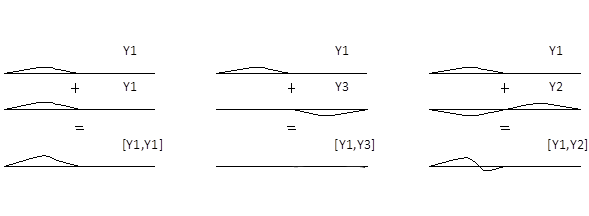
\includegraphics[scale=0.8]{fig2.png}
	\caption{Funciones de Forma Resultantes.}
	\label{fig:fig2}
\end{figure}

\end{document}
